\chapter{Prezentacja warstwy użytkowej}
\noindent Aplikacja posiada interfejs użytkownika w formie konsoli, umożliwiający:
\begin{itemize}
    \item Dodawanie i edycję pracowników,
    \item Rejestrowanie godzin pracy i ich zapis do plików tekstowych,
    \item Filtrowanie danych według wybranego zakresu czasu.
\end{itemize}

\noindent Przykładowe zrzuty ekranu aplikacji:
\begin{figure}[h]
    \centering
    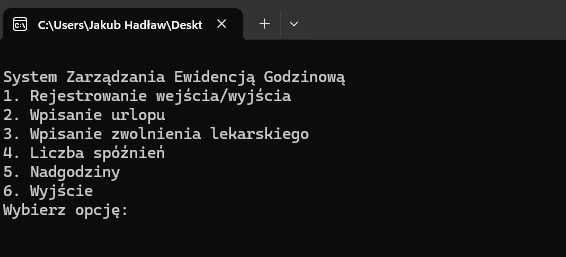
\includegraphics[width=0.8\textwidth]{ss1.png}
    \caption{Główne menu aplikacji}
\end{figure}

\begin{figure}[h]
    \centering
    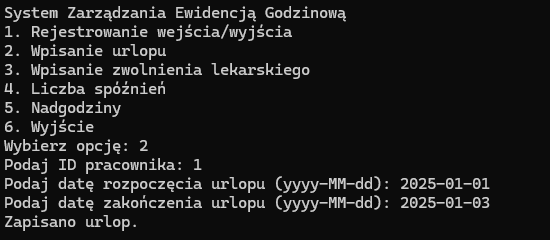
\includegraphics[width=0.8\textwidth]{ss2.png}
    \caption{Ewidencja godzin pracy}
\end{figure}
\begin{figure}[h]
    \centering
    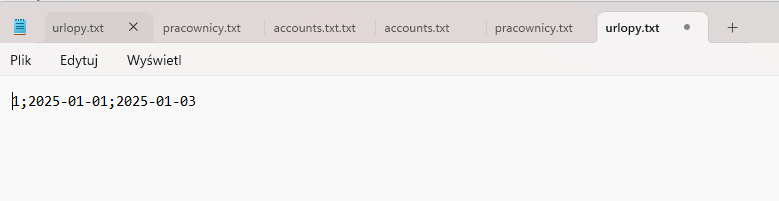
\includegraphics[width=0.8\textwidth]{ss3.png}
    \caption{Zapis w pliku tekstowym}
\end{figure}